%\epigraph{Yesterday's rose stands only in name, we hold only empty names.}{--- \textup{Umberto Eco}, \textit{The Name of Rose}}
This chapter introduces the properties of neutrinos and their interactions, focusing on the weak interactions, neutrino mass and flavor transformations. Existence of the particle (or class of particles) now known as the neutrino was first proposed by Pauli, to explain the (otherwise incomprehensible) spread of the electron energy spectrum in radioactive beta-decay. Since the first (indirect) {\em observations} of the neutrino, decades later in the 1950s, various types of neutrino experiments have measured and studied neutrinos produced from different sources: the core of the Sun, Earth's mantle and crust, the atmosphere, fission reactors, accelerator beams, and astrophysical objects such as supernovae. To state the obvious, these sources produce (in turn): solar neutrinos, geoneutrinos, atmospheric neutrinos, reactor antineutrinos, accelerator neutrinos and supernova/astrophysical neutrinos. Experiments focused on solar neutrinos have unraveled the phenomenon of neutrino flavor transformation in matter. The solar neutrino experiments relevant to the analysis presented in Chapter 6 are introduced. The last section of this chapter introduces the major physics goal for SNO+, i.e. neutrinoless double beta decay, and covers experiments relevant to that goal.

\section{Overview}

A neutrino is a neutral, spin-1/2 fermion that interacts ({\em with other fermions or fermionic fields}) only via the weak interaction and gravity. Its basic properties and interactions are described by the Standard Model (SM), a theory describing the properties of all elementary particles currently observed and their interactions based on {\em three} fundamental forces: the strong, weak, and electromagnetic forces. Notably the gravitational force, though equally deserving the adjective `fundamental', is not included in the Standard Model, and a longstanding effort to unify the four forces is ongoing. 

The SM has successfully explained and predicted phenomena in particle physics since the latter half of the 20th century. An important triumph achieved by the SM is the discovery of the predicted Higgs bosons in 2012. However, there are still open issues in the SM. Besides the question of accommodating gravity, some of the unsolved questions relate to the mysterious properties and behaviour of neutrinos: What are the masses of neutrinos? How do neutrinos obtain their masses? Why are their masses so small compared to those of the other elementary particles? Are neutrinos their own antiparticles? Still further questions about neutrinos are likely to emerge. Were any of these questions to be answered, a door would open to new physics theories beyond the SM.

Since neutrinos weakly interact with other particles and fields, they can penetrate through massive matter or travel a long way through space without being interrupted. Neutrinos produced in the core of the Sun, in Supernovae, or in the galactic core of the Milky Way can carry original information of these astrophysics objects and easily bring these information to the detectors on the Earth. This property enables neutrinos as a probe to study the status of astrophysics objects.

The interesting facts mentioned above put the researches of neutrinos under the spotlight. 

The existence of neutrinos was first put forward by Wolfgang Pauli in the 1930s to solve the observed contradicts in $\beta$-decay process. In 1914, James Chadwick found that the electrons emitted in $\beta$-decay (called the ``$\beta$-electrons'') have a continuous energy spectrum\cite{leite1996weak}. However, since nuclei have discrete energy levels, the energy spectrum of $\beta$-electrons should be discrete and equal to the difference between the final and initial states of nuclei. This indicates that the energy and momentum are not conserved if only nuclei and $\beta$-electrons present in the $\beta$-decay products. Pauli then introduced a charge-neutral, spin-1/2, and nearly massless particle to the $\beta$-decay products. This particle was later called ``neutrino'' (the small neutral one) by Enrico Fermi. The neutrinos take away a part of energies and then cause the broad energy spectrum of $\beta$-electrons, thus the problem was solved.

In 1934, Fermi developed the four-fermion vertex interaction theory to describe the weak interactions relating to neutrinos. Soon after that, Bethe and Peierls suggested direct neutrino detection can be made via a neutrino-induced interaction, called the inverse beta decay (IBD): $\bar{\nu}_e+p\to e^+ + n$. Their calculation showed that the IBD cross-section was in the order of $\mathcal{O}(10^{-44}$ cm$^2)$, which was difficult for detection\cite{bethe1934neutrino}. Though the task to detect neutrinos was difficult, in 1956, Fred Reines and Clyde Cowan made the first discovery of the antineutrinos from nuclear reactors. They measured the cross-section as $6.3\times10^{-44}$ cm$^2$, which was consistent with Bethe's calculation\cite{reines1960detection}.

In 1962, Lederman, Schwartz, and Steinberger demonstrated that more than one type of neutrino exists by detecting the interactions of the muon neutrino ($\nu_\mu$)\cite{danby1962observation}. The tau neutrino ($\nu_\tau$) was proposed after the discovery of the $\tau$ lepton and was observed in 2000 by the DONUT collaboration\cite{kodama2001observation}. The decay width of the $Z^0$ boson measured by the ALEPH collaboration implied that based on the SM, the number of light neutrino species is three\cite{decamp1989determination}.

Currently, there are three flavor neutrinos described in the SM. Neutrinos mostly participate in the weak interaction, while the other interactions are negligible. Via weak interaction, a neutrino $\nu_x$ is generated with a definite leptonic flavor, accompanied by one of the three charged leptons: electron ($e$), muon ($\mu$) or tauon ($\tau$), from which it is identified as an electron neutrino ($\nu_e$), a muon neutrino ($\nu_\mu$), or a tau neutrino ($\nu_\tau$). By observing the produced secondary
charged particles, neutrinos can be detected.

\section{Neutrino Interactions}\label{sect:nuInteraction}

In the SM, the weak interaction is described by the electroweak theory based on the Glashow-Weinberg-Salam (GWS) model, as fermions exchanging three types of gauge bosons, the weak force carriers: the charged $W^{\pm}$, and the neutral $Z^0$. The theory requires the lepton number and lepton flavor conservation and allows only the chiral left-handed neutrino ($\nu_L$) and right-handed antineutrino ($\bar{\nu}_R$) to participate in weak interactions. Neutrino interactions include the neutrino-electron scattering, neutrino-nucleon scattering and hadron decays \cite{giunti2007fundamentals}. 

This thesis studies solar neutrinos in the energy range $E_\nu\sim\mathcal{O}$(0.1-10 MeV), a range in which the most completely understood interactions are neutrino elastic scattering on electrons, protons and nuclei \cite{antonio2018state}, see Table.~\ref{tab:nuInteraction}. Elastic scattering can proceed via the charged weak current (CC) process entailing an exchange of the $W^\pm$ bosons, or via the neutral weak current (NC) process wherein the $Z^0$ boson is exchanged. In particular the elastic scattering interaction $\nu+e^-$ ES: $\nu_x + e^{-}\to\nu_x+e^-$ ($x=e,\mu,\tau$) plays an important role in the detection of solar neutrinos, and will be discussed in the next section.


\begin{table}
	\caption{Neutrino interactions in the $\mathcal{O}$(0.1-10 MeV) energy region, modified from Ref.~\cite{antonio2018state}.\label{tab:nuInteraction}}
	\begin{tabular*}{140mm}{ccc}
		\toprule 
		ES & IBD  & Nuclear Interactions\\
		\midrule
		$\overset{(-)}\nu_x+e^-\to \overset{(-)}\nu_x+e^-$ & $\bar{\nu}_e+p\to n+e^+$ & $\nu_e+(N,Z)\to(N-1,Z+1)+e^-$\\
		$\overset{(-)}\nu_x+p\to \overset{(-)}\nu_x+p$ &  & $\bar{\nu}_e+(N,Z)\to(N+1,Z-1)+e^+$\\
		& & $\nu_x+A\to \nu_x+A^*$\\
		& & $\nu_x+A\to \nu_x+A$\\
		\bottomrule	
	\end{tabular*}
\end{table}


\subsection{Neutrino-Electron Elastic Scattering}\label{sect:NuEStheory}
The $\nu+e^-$ ES process is a pure leptonic process and can be precisely described by the electroweak theory in the SM. This process has no energy threshold, and is sensitive to all neutrino flavors. It is valid for both neutrino and antineutrino.

The amplitude for this process has contributions from both NC and CC interactions. Fig.~\ref{fig:feynman-es} shows the tree-level Feynman diagrams (without radiative corrections) for the CC ES (Fig.~\ref{fig:feynman-es:a}) and the NC ES (Fig.~\ref{fig:feynman-es:b}) interactions. 

It is a characteristic of the charged vertex that lepton generation does not change, thus, although the $\nu_e$ can undergo both the CC ES and NC ES interactions, the $\nu_{\mu}$ and $\nu_\tau$ may interact only through the NC ES interaction\footnote{For $\bar{\nu}_e$, the Feynman diagram of the CC ES is a s-channel diagram rather than the t-channel presented in Fig~\ref{fig:feynman-es:a}}. In other words for the CC channel the charged lepton in the final state must belong to the same lepton generation as the (incoming) neutrino, this being required by (the theory of) the weak interaction. In this case, since the rest masses of muon and tau leptons are much larger than the masses of solar neutrinos, specifically $m_\mu\approx 105.6$ MeV and $m_\tau\approx 1.78$ GeV \cite{pdg2020}, evaluation of the elastic scattering via the CC channel requires energy thresholds larger than 10.9 GeV for the $\nu_\mu$ and 3089 GeV for the $\nu_\tau$, which is impossible for solar neutrinos. On the other hand, for the NC ES, the Feynman diagram is the same for all flavors $\bar{\nu}_x$\cite{giunti2007fundamentals,xing2011neutrinos}. 

\begin{figure}[htbp]
	\centering
	\subfigure[CC ES.\label{fig:feynman-es:a}]{ 
	\begin{minipage}[b]{0.4\textwidth}
		\centering %\label{fig:feynman-es:CC_ES}
		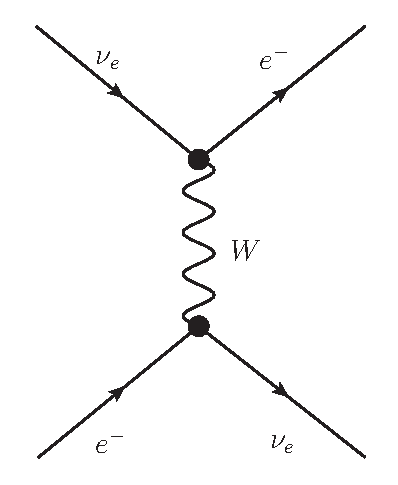
\includegraphics[height=4.5cm]{charged.eps}
	\end{minipage}
}
	\subfigure[NC ES.\label{fig:feynman-es:b}]{ 
	\begin{minipage}[b]{0.35\textwidth}
	\centering % \label{fig:feynman-es:NC_ES}
	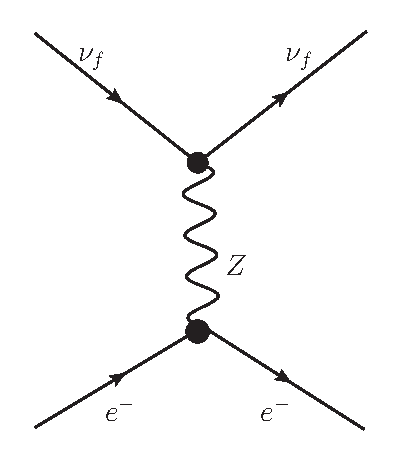
\includegraphics[height=4.5cm]{neutral.eps}
    \end{minipage}
}
	\caption[Feynman diagrams for the elastic scattering interaction in different channels at tree level.]{Feynman diagrams for the elastic scattering interaction in different channels at tree level. (a): CC ES for $\nu_e$; (b): NC ES for all flavors $\nu_x$ ($x=e,\mu,\tau$).\label{fig:feynman-es}}
\end{figure}
%	\begin{minipage}[t]{0.45\textwidth}{(b)}
%	\centering
%	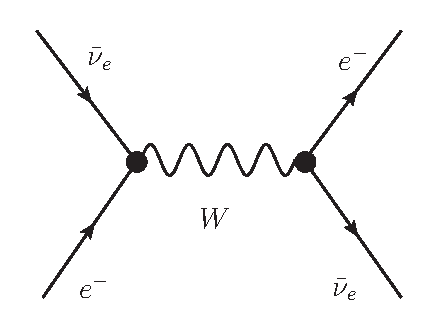
\includegraphics[width=5cm]{charged_antiNu.eps}
%\end{minipage}


In a particle detector, the `target' electron is normally an atomic electron of the detector medium, and is considered to be at rest in the laboratory frame. The incoming solar neutrinos interact with these electrons via the $\nu+e^-$ ES, and these electrons are scattered, as shown in Fig~\ref{fig:ESdiagram}. 

\begin{figure}[htbp]
	\centering	
	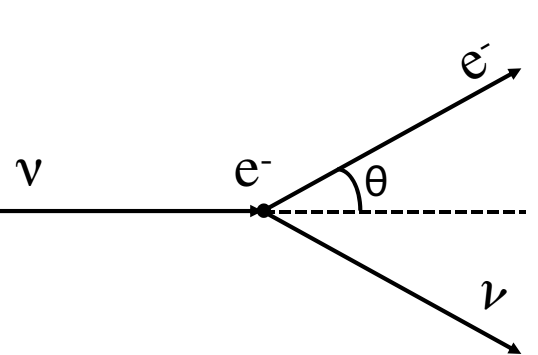
\includegraphics[width=6cm]{ElasticScatteringCartoon.png}
	\caption[A diagram of the $\nu + e^-$ elastic scattering in the lab frame.]{A diagram of the $\nu + e^-$ elastic scattering in the lab frame, modified from Ref.~\cite{giunti2007fundamentals}.	\label{fig:ESdiagram}}
\end{figure}

In the laboratory frame, the kinetic energy of a recoil electron from the $\nu+e^-$ ES process is \cite{giunti2007fundamentals}:
\begin{equation}\label{eq:Te_scattered_electron}
T_e = \frac{2m_e c^2 E_\nu^2\cos^2\theta}{(m_e c^2 +E_\nu)^2-E_\nu^2\cos^2\theta},
\end{equation}
where the scattering angle $\theta$ is defined (Fig.~\ref{fig:ESdiagram}) as the deviation of the outgoing (scattered) electron's path and the path of the incoming neutrino (Eqn.~\ref{eq:Te_scattered_electron} follows directly from conservation of relativistic 4-momentum, if one neglects the mass of the neutrinos). The recoil electron has maximum energy 
\begin{equation}
T_{max}=\frac{2E^2_\nu}{2E_\nu+m_e c^2} 
\end{equation}
when it scatters along the direction of the incident neutrino (i.e. when $\theta=0$ or $\theta=\pi$).

The direction of the scattered electron is strongly correlated with the direction of the incident neutrino. For solar neutrinos, the scattering angle (relative to the axis between the Snoplus detector and the sun's position) is denoted as ``solar angle'' ($\theta_{sun}$) in this thesis. It is one of the crucial parameters for measuring solar neutrinos, which will be discussed in Chapter 6 for analyzing solar neutrinos in the SNO+ water phase. By rearranging Eqn.~(\ref{eq:Te_scattered_electron}) we obtain
\begin{eqnarray}\label{eq:costhetaSun}
\cos\theta_{sun} &=& \sqrt{\frac{T_e(m_e c^2 + E_\nu)^2}{2m_e c^2 E_\nu^2+T_eE_\nu^2}} \; , \nonumber \\
                 &\;& \\
                 &=& \left( 1 + \frac{m_e c^2}{E_{\nu}} \right) \; \frac{1}{\sqrt{1 + \frac{2 m_e c^2}{T_e}}} \; \nonumber.
\end{eqnarray}

The differential cross-section of the $\nu+e^-$ ES in the lab frame (without radiative corrections) is given by\cite{giunti2007fundamentals,xing2011neutrinos,suzuki2020sun}:
\begin{equation}
\frac{d\sigma}{dT_e}(E_\nu,T_e)=\frac{G_F^2m_e}{2\pi}\left[(c_V+c_A)^2+(c_V-c_A)^2\left(1-\frac{T_e}{E_\nu}\right)^2-(c_V^2-c_A^2)\frac{m_eT_e}{E_\nu^2}\right],
\end{equation}
where $G_F$ is the Fermi coupling constant in the weak interaction; the coupling parameters $c_V=2\sin^2\theta_W\pm\frac{1}{2}$, $c_A=\pm\frac{1}{2}$, and the ``$+$'' sign is for the $\nu_e+e^-$ case while ``$-$'' sign is for the $\nu_{\mu,\tau}+e^-$ cases; the Weinberg angle $\sin\theta_W$ is given by $\sin^2\theta_W=0.23$. The cross-section is $\sigma^{ES}(\nu_e +e^-)=9.52\times 10^{-44}~(E_\nu/10~\mathrm{MeV)~cm^2}$ and the expected solar neutrino rate is (see \cite{suzuki2020sun}):
\begin{equation}
R=A \, \int\limits_{T_{thresh}}^{T_{max}} \, \frac{d\sigma}{dE} \, \frac{dN}{dE_\nu} \, dE_\nu\; .
\end{equation}
The shape of the recoil electron energy spectrum and the directionality are utilized by the experiments to tag solar neutrinos in real-time \cite{suzuki2020sun}. These experiments will be introduced in Sect.~\ref{sect:solarNu}.

For the solar neutrino case, $E_\nu\gg m_e c^2$, the total cross-section of $\nu_e+e^-$ ES and $\nu_x+e^-$ ES ($x=\mu$ or $\tau$) can safely be approximated as \cite{xing2011neutrinos}:
\begin{eqnarray}
\sigma^{ES}(\nu_e+e^-) &=& \frac{2G_F^2}{\pi}m_e E_\nu \left[(1+c_L)^2+\frac{1}{3}(c_R)^2\right],\\
\sigma^{ES}(\nu_x+e^-) &=& \frac{2G_F^2}{\pi}m_e E_\nu \left[(c_L)^2+\frac{1}{3}(c_R)^2\right],
\end{eqnarray}
where $x=\mu$ or $\tau$, $c_L=\frac{(c_V+c_A)}{2}$ and $c_R = \frac{(c_V-c_A)}{2}$. Then the ratio of $\sigma^{ES}(\nu_{\mu,\tau}+e^-)$ to $\sigma^{ES}(\nu_e+e^-)$ is \cite{xing2011neutrinos}:
\begin{equation}\label{eq:ratio1}
\frac{\sigma^{ES}(\nu_{x}+e^-)}{\sigma^{ES}(\nu_e+e^-)} = \frac{3(c_L)^2+({c_R})^2}{3(1+c_L)^2+(c_R)^2} \approx 0.155 \; .
\end{equation}
Thus the cross-section for CC ES is about 6.5 times larger than that for NC ES. It follows that {\em if} at the detector the fluxes of $\nu_e$ ($\Phi_{\nu_e}$) and of $\nu_{\mu}$ {\bf or} $\nu_\tau$ ($\Phi_{\nu_x}$) {\em were equal}, the expected number of $\nu_e$ detected would be about 6.5 times greater than the sum of the $\nu_{\mu}$ and $\nu_\tau$ events. This theory-based expectation was an input in the solar neutrino simulations, which will be discussed in Sect.~\ref{sect:evaluateFlux}, Chapter 6. 

%This indicates that for the experiments measuring the $\nu$ via the $\nu e^-$ ES channel, for the same exposure (detector running time$\time$ active target mass), the number of the measured $\nu_e$ is about 6.5 times the number of $\nu_\mu$ or $\nu_\tau$.

\section{Neutrino Flavor Transformation}
Neutrino flavor transformation is a quantum mechanical interference phenomenon \cite{akhmedov2019quantum}. It was first discovered in 1998, based on the analysis of atmospheric neutrino fluxes measured by the Super-Kamiokande (Super-K) experiment to solve the ``atmospheric neutrino anomaly'' \cite{fukuda1998evidence}. It is the first direct evidence showing that neutrinos have finite masses and that the SM is incomplete.

\subsection{Vacuum Oscillation}\label{sect:VacuumOsci}
For neutrino flavor oscillation experiments, neutrinos are detected in certain flavor eigenstates via weak interaction. A neutrino flavor state vector can be taken as a linear superposition of the mass eigenstates. For three-flavor neutrino mixing, we have\footnote{The reader is asked to be alert for two distinct usages of $i$ --- as both $i=\sqrt{-1}$ and as an {\em index}. Short of invoking unusual symbols, such conflicts are hard to avoid. Hopefully no confusion will arise.} \cite{pdg2020}:
\begin{equation}\label{eq:mixingmatrix}
|\nu_f\rangle = \sum_{j=1}^3U^*_{fj}|\nu_j\rangle, 
\end{equation}
where $f=(e,\mu,\tau)$ and $j=(1,2,3)$. The unitary matrix $U^*_{fj}$, known as the Pontecorvo– Maki– Nakagawa– Sakata (PMNS) matrix, $U_{PMNS}$, can be parameterized as\footnote{Here we ignore the Majorana CP violation phases, which cancel out and do not affect the calculation of flavor transformation probability. They will be introduced in Sect.~\ref{sect:doublebeta}.}: 
\begin{equation}\label{eq:uPMNS}
U_{PMNS} =
\begin{pmatrix}
1 &0 &0\\
0 &c_{23} &s_{23}\\
0 &-s_{23} &c_{23}\\ 
\end{pmatrix}
\begin{pmatrix}
c_{13} &0 &e^{-i\delta_{CP}}s_{13}\\
0 &1 &0\\
e^{-i\delta_{CP}}s_{13} &0 &c_{13}\\ 
\end{pmatrix}
\begin{pmatrix}
c_{12} &s_{12} &0\\
-s_{12} &c_{12} &0\\
0 &0 &1\\ 
\end{pmatrix},
\end{equation}
where $c_{jk}\equiv \cos\theta_{jk}$ and $s_{jk}\equiv \sin\theta_{jk}~(j,k = 1,2,3)$. In the PMNS matrix, there are four parameters: the three mixing angles $\theta_{12}$, $\theta_{13}$, $\theta_{23}$ and the charge-parity (CP) violation parameter of the lepton sector, $\delta_{CP}$. The unknown value of $\delta_{CP}$ is related to leptogenesis, the hypothetical physical process that produced an asymmetry between leptons and anti-leptons in the very early universe \cite{wiki_cp}. 

Now consider the propagation of a neutrino in the vacuum. Suppose that a neutrino is generated at time $t_0=0$ (in the lab frame) by some mechanism (source), and that it is in flavor state
\begin{equation}
|\nu(0) \rangle = |\nu_\alpha \rangle = \sum_j U^*_{\alpha j}|\nu_j \rangle \;.
\end{equation}
The energy of the initial state is a linear combination of the energies $E_j=\sqrt{p_j^2 + (m_j c^2)^2}$ of the mass eigenstates (where $p_j$ is the 3-momentum). The neutrino then propagates in vacuum with a speed close to the speed of light (ultra-relativistic) for a distance $L$ and is finally detected at time $t$ in a detector.

Now assume that the 3-momentum vector is oriented along the vector separating source and detector, with a single non-zero component. Via the 1D Schr\"{o}dinger equation, the amplitude for the flavor eigenstate $|\nu_\beta\rangle$ in the detector at $(L,t)$ is (using the natural units: $\hbar=c=1$) \cite{aitchison2012gauge}:
\begin{equation}
\mathcal{A}(\nu_\alpha\to\nu_\beta;L,E)=\sum_{j}U^*_{\alpha j}e^{-i E_j t+i p_j L}\langle\nu_\beta|\nu_j,p_j\rangle=\sum_{j}U^*_{\alpha j}U_{\beta j}e^{-iE_jt+ip_jL} \; .
\end{equation}
Then the probability that the neutrino $\nu_\alpha$ at time $t_0=0$ transforms into a $\nu_\beta$ at time $t$ is:
\begin{equation}\label{oscillationEq1}
 \begin{split}
&P(\nu_\alpha\to\nu_\beta;L,E)= |\mathcal{A}|^2 \; = \; \mathcal{A} \mathcal{A}^* \, =  \\%|\langle\mathcal{A}(\nu_\alpha\to\nu_\beta;L,E)|\mathcal{A}(\nu_\alpha\to\nu_\beta;L,E)\rangle|^2=\\
&(U^*_{\alpha 1}U_{\beta 1}e^{-iE_1t+ip_1L}+U^*_{\alpha 2}U_{\beta 2}e^{-iE_2t+ip_2L}+...)(U_{\alpha 1}U^*_{\beta 1}e^{+iE_1t-ip_1L}+U_{\alpha 2}U^*_{\beta 2}e^{+iE_2t-ip_2L}+...)=\\
&\sum_j |U_{\alpha j}|^2|U_{\beta j}|^2 + \sum_{j>k}(U^*_{\alpha j}U_{\beta j}U_{\alpha k}U^*_{\beta k})\exp\{-i(E_j-E_k)t+i(p_j-p_k)L\}+(j\leftrightarrow k),
\end{split}
\end{equation}
where $(j\leftrightarrow k)$ stands for the second term exchanging the $j,k$ indices.

For the second term in Eqn.~\ref{oscillationEq1}, in the ultra-relativistic case, $p_j\simeq p_k\equiv p\simeq E\gg m$, where $E$ is the average energy\footnote{Note: here and elsewhere in the thesis factors of $c$ or $c^2$ (etc.) will be dropped -- but are understood to be necessary for dimensional homogeneity.}. Then $E_j=\sqrt{p^2_j+m^2_j}\simeq p+\frac{m_j^2}{2E}$ and thus \cite{pdg2020,aitchison2012gauge}
\begin{equation}
E_j-E_k\simeq \frac{m^2_j-m^2_k}{2E}\equiv \frac{\Delta m^2_{jk}}{2E} \; .
\end{equation}
Here $\Delta m^2_{jk}$ is a set of parameters called the `mass square differences', and they feature in the flavor transition probability\footnote{Viewed as a matrix or rank-2 tensor, the quantity $\frac{\Delta m^2_{jk}}{2E}$ has zeros along the diagonal. It is anti-symmetric in its indices.}. With the further simplification that $L\simeq ct=t~(c\equiv 1)$, we obtain
\begin{equation*}
\exp\{-i(E_j-E_k)t+i(p_j-p_k)L\}\simeq \exp\{-i\frac{\Delta m^2_{jk}}{2E} \, L\} \; .
\end{equation*}
In addition,
\begin{eqnarray*}
U^*_{\alpha k}U_{\beta j}U_{\alpha k}U^*_{\beta k} &=& |U^*_{\alpha j}U_{\beta j}U_{\alpha k}U^*_{\beta k}| \, \exp\{i\phi_{\alpha\beta;jk}\} \; ,\\
&=& |U^*_{\alpha j}U_{\beta j}U_{\alpha k}U^*_{\beta k}| \; \{ \cos \phi_{\alpha\beta;jk} + i \sin \phi_{\alpha\beta;jk}\}
\end{eqnarray*}
where 
\begin{eqnarray*}
\phi_{\alpha\beta;jk} &=& \mathrm{Arg}(U^*_{\alpha j}U_{\beta j}U_{\alpha k}U^*_{\beta k}) \; , \\
\phi_{\alpha\beta;jk} &=& -\phi_{\alpha\beta;kj} \; .
\end{eqnarray*}
Then combining the second term (of Eqn.~\ref{oscillationEq1}) and the corresponding $(j\leftrightarrow k)$ term, Eqn.~\ref{oscillationEq1} can be written as \cite{aitchison2012gauge}:
\begin{equation}\label{oscillationEq2}
P_{\nu_\alpha\to\nu_\beta}(L,E)=
\sum_j |U_{\alpha j}|^2|U_{\beta j}|^2 + 2\sum_{j>k}|U^*_{\alpha j}U_{\beta j}U_{\alpha k}U^*_{\beta k}|\cos(\frac{\Delta m^2_{jk}}{2E}L-\phi_{\alpha\beta;jk}),
\end{equation}
where (recall) $L$ is distance from source to detector, and $E$ is the energy of the neutrino {\em averaged along the path}.

Because the matrix $U$ is unitary the second term in Eqn.~\ref{oscillationEq2} expands as
\begin{equation}
 \begin{split}
&|U^*_{\alpha j}U_{\beta j}U_{\alpha k}U^*_{\beta k}|\{\cos(\phi_{\alpha\beta;jk})\cos(\frac{\Delta m^2_{jk}}{2E}L)+\sin(\phi_{\alpha\beta;jk})\sin(\frac{\Delta m^2_{jk}}{2E}L)\}=\\
&\Re(U^*_{\alpha j}U_{\beta j}U_{\alpha k}U^*_{\beta k})(1-2\sin^2\frac{\Delta m^2_{jk}L}{4E})+\Im(U^*_{\alpha j}U_{\beta j}U_{\alpha k}U^*_{\beta k})\sin\frac{\Delta m^2_{jk}L}{2E},
 \end{split}
\end{equation}
and when $t=L=0$, Eqn.~\ref{oscillationEq2} becomes
\begin{equation}
P_{\nu_\alpha\to\nu_\beta}=\delta_{\alpha\beta}=\sum_j |U_{\alpha j}|^2|U_{\beta j}|^2+2\sum_{j>k}\Re(U^*_{\alpha j}U_{\beta j}U_{\alpha k}U^*_{\beta k}) \; .
\end{equation} 
We can now eliminate the first term in Eqn.~\ref{oscillationEq2}, and upon doing so we obtain the important and widely cited `vacuum neutrino oscillation equation'\cite{pdg2020,aitchison2012gauge}:
\begin{eqnarray}\label{common_oscillation}
P_{\nu_\alpha\to\nu_\beta}(L,E) = \delta_{\alpha\beta} &-& 4\sum_{j>k} \Re[U_{\beta j}U^*_{\alpha j}U_{\alpha k}U^*_{\beta k}]\sin^2\frac{\Delta m^2_{jk}L}{4E} \nonumber\\
&\;& \\
&+& 2\sum_{j>k} \Im(U_{\beta j}U^*_{\alpha j}U_{\alpha k}U^*_{\beta k})\sin\frac{\Delta m^2_{jk}L}{2E} \nonumber \, .
\end{eqnarray}

Choosing a set of units commonly used by experiments and with dimensional transformation, we have \cite{pdg2020}:
\begin{equation}\label{oscillationCondition}
X_{jk}\equiv \frac{\Delta m^2_{jk}L}{4E}=\frac{1.267\Delta m_{jk}^2[\mathrm{eV}^2]L[\mathrm{m}]}{E_\nu[\mathrm{MeV}]}.
\end{equation}
Maximum oscillation occurs when $X_{jk}\sim \pi$, which gives an effective length $L^{osc}(\Delta m_{jk},E_\nu)=4\pi E/|\Delta m_{jk}^2|$.

Currently, the four parameters in the PMNS matrix ($\theta_{12},\theta_{13},\theta_{23}$ and $\delta_{CP}$), as well as the two squared-mass differences: $\Delta m^2_{21}=m_2^2-m_1^2$ and $\Delta m^2_{32}=m^2_3-m^2_2$, have been measured by neutrino oscillation experiments. 

These experiments can be classified by the neutrino sources they use: the sun, nuclear reactors, muons generated in the atmosphere by cosmic rays, particle accelerators, and, astronomical sources in deep space. Table~\ref{nu_exp} lists the energy scale of the neutrino source as well as the example experiments.

\begin{table}[ht]
	\caption{Neutrino experiments for studying flavor transformation.\label{nu_exp} }	
	{\centering
		\begin{tabular*}{135mm}{c@{\extracolsep{\fill}}cccc}
			\toprule 
			type & source & $E_\nu$ & example\\
			\midrule
			solar& the Sun & MeV scale & SNO \\
			reactor& reactor & MeV scale & DayaBay \\
			atmospheric& cosmic-ray& GeV scale & SuperK\\
			accelerator&  $\nu$ beam from accelerator & GeV scale & T2K\\	
			astronomical& astronomical objects & GeV-EeV scale & IceCube\\
			\bottomrule	
		\end{tabular*}
	}
\end{table}

Currently, the sign of $\Delta m^2_{32}$ is still not determined. If it is positive, the neutrino masses are in a `normal hierarchy' (NH, $m_3>m_2>m_1$); otherwise they are in an inverted hierarchy (IH, $m_3<m_1<m_2$) \cite{pdg2020}. 

For $\Delta m^2_{21}$ and $\theta_{12}$, a combined analysis of the measurements from the reactor experiment KamLAND (Kamioka Liquid Scintillator Antineutrino Detector) and the solar neutrino experiment SNO (Sudbury Neutrino Observation) gave $\Delta m^2_{21} = 7.59^{+0.21}_{-0.21}\times 10^{-5} \; \mathrm{eV}^2$ and $\tan^2{\theta}_{21}=0.47^{+0.06}_{-0.05}$ \cite{abe2008precision}. Details will be discussed in Sect.\ref{sect:solarNu}.

Accelerator neutrino experiments as well as atmospheric neutrino experiments have measured $\Delta m^2_{32}$ and $\theta_{23}$. The most recent results from Super-K show that assuming a normal mass hierarchy, $\Delta m^2_{32} = 2.5^{+0.13}_{-0.20}\times 10^{-3} \, \mathrm{eV}^2$ and $\sin^2\theta_{23}=0.588^{+0.031}_{-0.064}$ \cite{abe2018atmospheric}. 

In 2012, the reactor neutrino experiment Daya Bay reported the discovery of non-zero $\theta_{13}$ with a significance of 5.2$\sigma$. In 2016, Daya Bay reported that $\sin^2 2\theta_{13} = 0.0841\pm0.0027(stat.)\pm0.0019(syst.)$. This high-precision result makes $\sin^2 2\theta_{13}$ the best measured mixing angle \cite{an2017measurement,qian2019physics}.

In the case of antineutrino flavor oscillation, we have $|\bar{\nu}_\alpha\rangle=\sum_i U_{\alpha i}|\bar{\nu}_i,p_i\rangle$. By a calculation analogous to that summarized above, a similar oscillation probability equation can be obtained, but with the final term (in \ref{common_oscillation}) being negative \cite{aitchison2012gauge}:
\begin{eqnarray}\label{antiNu_eq1}
P_{\bar{\nu}_\alpha\to\bar{\nu}_\beta}(L,E)=\delta_{\alpha\beta} &-& 4\sum_{j>k} \Re[U_{\beta j}U^*_{\alpha j}U_{\alpha k}U^*_{\beta k}]\sin^2\frac{\Delta m^2_{jk}L}{4E} \nonumber\\
&\;& \\
&-& 2\sum_{j>k} \Im(U_{\beta j}U^*_{\alpha j}U_{\alpha k}U^*_{\beta k})\sin\frac{\Delta m^2_{jk}L}{2E} \nonumber \, .
\end{eqnarray}

This provides a measure of CP violation \cite{aitchison2012gauge},
\begin{equation}\label{cpV_eq1}
%\begin{split}
\mathcal{A}_{CP}=P_{\nu_\alpha\to\nu_\beta}(L,E)-P_{\bar{\nu}_\alpha\to\bar{\nu}_\beta}(L,E)=
4\sum_{j>k} \Im(U_{\beta j}U^*_{\alpha j}U_{\alpha k}U^*_{\beta k})\sin\frac{\Delta m^2_{jk}L}{2E},
%\end{split}
\end{equation}
where $\delta_{CP}$ is examined by the experiments which measure the difference between neutrino and antineutrino oscillation probabilities $P(\bar{\nu}_\alpha\to\bar{\nu}_\beta)$ and $P(\nu_\alpha\to\nu_\beta)$ \cite{xing2011neutrinos}. In 2019, the Tokai-to-Kamioka (T2K) experiment in Japan claimed confidence intervals for $\delta_{CP}$ with three standard deviations ($3\sigma$): [-3.41,-0.03] (NH) or [-2.54,-0.32] (IH). This result indicates that leptons exhibit CP violation \cite{abe2019constraint}.

\subsection{Matter Effect}\label{sect:MSW}

The matter effect is caused by neutrinos interacting with ambient electrons and nucleons in dense matter such as the Sun or the Earth. In this case, at the MeV energy scale, the $\nu+e^-$ ES is dominant. As explained in Sect.~\ref{sect:NuEStheory}, a $\nu_e$ may interact electrons via either the charged current (CC) or the neutral current (NC) mechanism, while $\nu_\mu$ and $\nu_\tau$ interact only by the NC. Thus the $\nu_e+e^-$ ES has an additional potential, $V_{CC} =\sqrt{2} \, G_F \, n_e$, where $n_e$ is the number density of electrons in the matter encountered. This term alters the oscillation probabilities for neutrinos propagating in matter relative to the situation in the vacuum, an effect which is called the Mikheyev-Smirnov-Wolfenstein (MSW) mechanism \cite{smirnov2016solar,smirnov2005msw}.

In vacuum two-flavor mixing, the Schr\"{o}dinger equation can be written (in natural units) \cite{xing2011neutrinos}:
\begin{equation}\label{eq:2flavor_simple}
	i\frac{d}{dt}\begin{pmatrix}
		\nu_e\\
		\nu_\mu\\
	\end{pmatrix}
	=
	H^f_0
	\begin{pmatrix}
		\nu_e\\
		\nu_\mu\\
	\end{pmatrix},
\end{equation}
where
\begin{equation} \label{eq:H0f}
\begin{aligned}
 H^f_0 = \frac{1}{2E}\begin{pmatrix}m^2_1\cos^2\theta+m^2_2\sin^2\theta & (m^2_2-m^2_1)\sin\theta\cos\theta \\ (m^2_2-m^2_1)\sin\theta\cos\theta & m^2_1\sin2\theta+m^2_2\cos^2\theta\end{pmatrix} =
\\
\frac{\Delta m_{21}^2}{4E}\begin{pmatrix}
	-\cos 2\theta & \sin 2\theta\\
	\sin 2\theta & \cos 2\theta\\
\end{pmatrix}+\frac{(m_1^2+m_2^2)}{4E}\begin{pmatrix}
	1 & 0\\
	0 &1\\
\end{pmatrix},
\end{aligned}
\end{equation}
and $\Delta m^2_{21}=(m^2_2 - m^2_1)$.

To simplify the calculation, we can drop the second unitary term of $H^f_0$ that is irrelevant to the neutrino flavor transformation. Including the matter effect
\begin{equation}\label{eq:Hm}
	H_m = \begin{pmatrix}
		-\frac{\Delta m_{21}^2}{4E}\cos 2\theta+\sqrt 2G_Fn_e & \frac{\Delta m_{21}^2}{4E}\sin 2\theta\\
		\frac{\Delta m_{21}^2}{4E}\sin 2\theta &\frac{\Delta m_{21}^2}{4E}\cos 2\theta\\
	\end{pmatrix} \; .
\end{equation}
By analogy with mixing in vacuum, a mixing angle in matter, $\theta_m$ is defined as
\begin{equation}\label{eq:thetaM}
	\tan 2\theta_m = \frac{\Delta m^2\sin2\theta}{\Delta m^2\cos2\theta-2\sqrt 2E G_Fn_e},
\end{equation}
and an effective squared-mass difference in matter, $\Delta m^2_m$ is defined as:
\begin{equation}
	\Delta m^2_m = \sqrt{(\Delta m^2\cos2\theta - 2\sqrt 2EG_Fn_e)^2+(\Delta m^2\sin2\theta)^2}.
\end{equation}
Thus we can write the mixing equation relating the energy eigenstates in matter ($\nu_{1m},\nu_{2m}$) to the flavor eigenstates by a unitary matrix:
\begin{equation}\label{eq:matter_mixing}
	\begin{pmatrix}
		\nu_e\\
		\nu_\mu\\
	\end{pmatrix}
	= \begin{pmatrix}
		\cos\theta_m & \sin\theta_m\\
		-\sin\theta_m & \cos\theta_m \\
	\end{pmatrix}
	\begin{pmatrix}
		\nu_{1m}\\
		\nu_{2m}\\
	\end{pmatrix}.
\end{equation}

The probability of flavor transformation in matter is:
\begin{equation}
	P_{\nu_e\to\nu_{\mu}}=\sin^2(2\theta_m)\sin^2\Big(\frac{\Delta m_m^2L}{4E}\Big).
\end{equation}

The denominator in equation (\ref{eq:thetaM}) implies a resonance condition:
\begin{equation}\label{eq:reson_condition}
	V(n_e)=\sqrt 2G_Fn_e=\frac{\Delta m^2\cos2\theta}{2E}.
\end{equation}
From this condition, for a given $E$, there is a resonance density $n^{\mathrm{res}}_e$ while for a given $n_e$, there is a resonance energy $E^{\mathrm{res}}$. When the resonance condition is satisfied, $\theta_m = \frac{\pi}{4}$ and two flavor neutrinos are maximally mixed, even if the vacuum mixing angle $\theta$ is small. This is called matter enhanced neutrino oscillation \cite{smirnov2016solar,fukugita2013physics}. The matter effect was first observed by measuring the solar neutrino fluxes, which will be discussed in the next section.

\section{Solar Neutrinos}\label{sect:solarNu}

In the 1930s, Gamow, von Weizs{\"a}cker and Bethe et al. explained that the Sun's energy is derived from a series of nuclear reactions \cite{bethe1939energy}. Our current knowledge of these nuclear reactions has been summarized in the Standard Solar Model (SSM). 

The SSM is a modern and broadly accepted theory for tracing the evolution of the Sun from its beginning, which is based on contemporary data from theories and experimental measurements, including an equation of state describing the balance between the gravitational and pressure forces; the cross-sections of the nuclear reactions; and the modern Sun's mass, age, radius, luminosity, etc. \cite{haxton2013solar}. According to the SSM, the energy in the Sun is mainly produced by two sets of reactions: the proton-proton (pp) chain, which is dominant and contributes $\sim 98.6\%$ of the energy released, and the Carbon-Nitrogen-Oxygen (CNO) cycle, which contributes $\sim 1.4\%$ \cite{antonio2018state}. Fig.~\ref{fig:ppChain} shows all the reactions in the pp chain, and Fig.~\ref{fig:CNOcycle} shows the reactions in the CNO cycle. 

\begin{figure}[htbp]
	\centering	
	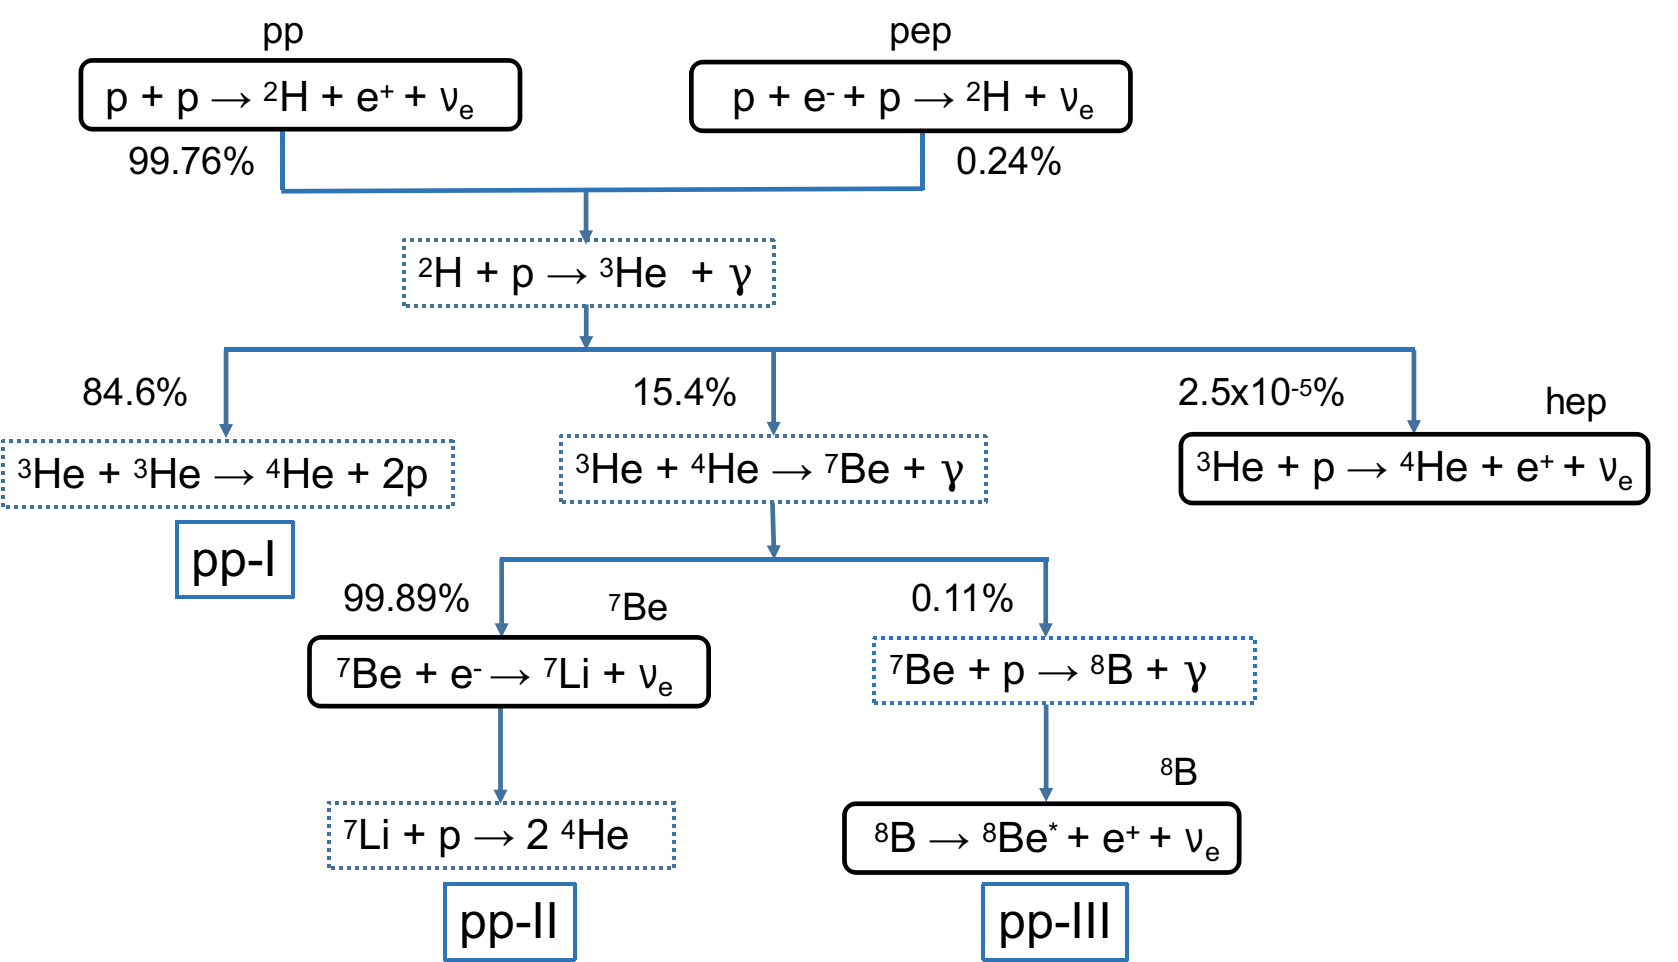
\includegraphics[width=14cm]{ppChain.png}
	\caption[All reactions in the three PP chains.]{All reactions in the three PP chains: PP-I, PP-II, PP-III. The reactions producing neutrinos are labeled in the solid frames. Modified from \cite{oberauer2020solar}.	\label{fig:ppChain}}
\end{figure}

\begin{figure}[htbp]
	\centering	
	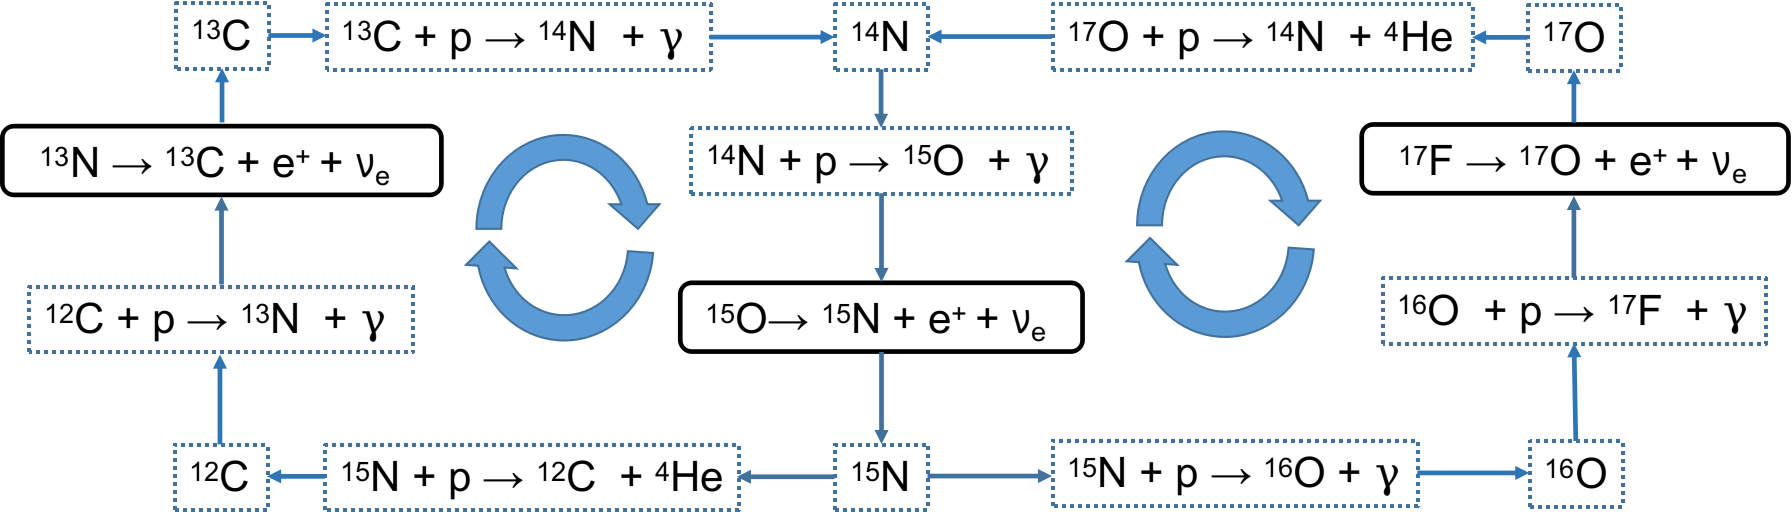
\includegraphics[width=14cm]{CNOcycle.png}
	\caption[All reactions in the CNO bicycle.]{All reactions in the CNO bicycle. The reactions producing neutrinos are labeled in the solid frames. Modified from \cite{oberauer2020solar}.	\label{fig:CNOcycle}}
\end{figure}

Via these nuclear reactions, hydrogen is eventually fused into helium, and the net nuclear transformation is $4p+2e^-\to^{4}$He $+2\nu_e+Q$, where the released energy $Q=26.73$ MeV is mostly in the form of the kinetic energy of the photons, with a small fraction carried by neutrinos \cite{antonio2018state,valle2015neutrinos}.

The electron neutrinos $\nu_e$ produced in the solar nuclear reactions are called ``solar neutrinos'' and they can be detected on the Earth. Due to the branching ratios and unterminated chains in the pp chain and CNO cycle, the solar neutrinos come from different reactions, as shown in Fig.~\ref{fig:ppChain} and Fig.~\ref{fig:CNOcycle}. They are named after the corresponding reactions, as shown in Table.~\ref{tab:solarNu}.

\begin{table}[htp]
	\caption[The main reactions producing solar neutrinos.]{The main reactions producing solar neutrinos in pp chain (a) and CNO cycle (b).\label{tab:solarNu} }	
	\subfigure[pp chain]{
		\begin{tabular*}{65mm}{cc}
			\toprule 
			solar $\nu_e$ & reaction  \\
			\midrule
			pp & $p+p\to ^2$H $+e^++\nu_e$ \\
			pep & $p+e^-+p\to^2$H $+~\nu_e$ \\
			hep &  $^3$He $+~p\to^4$He $+~e^++\nu_e$ \\ 
			$^7$Be &  $^7$Be $+~e^-\to^7$Li $+~\nu_e$\\
			$^8$B & $^8$B$\to^8$Be$^*+e^++\nu_e$\\
			\bottomrule	
		\end{tabular*}
	}
	\subfigure[CNO cycle]{
		\begin{tabular*}{65mm}{cc}
			\toprule 
			solar $\nu_e$  & reaction \\
			\midrule
			CNO &$^{13}$N$\to^{13}$C$+e^++\nu_e$\\	
			& $^{15}$O$\to^{15}$N$+e^++\nu_e$ \\
			& $^{17}$F$\to^{17}$O$+e^++\nu_e$ \\
			\bottomrule	
		\end{tabular*}
	}
\end{table}

The average energy of a solar electron neutrino ($\nu_e$) is calculated by summing over the energies $E^i_{\nu_e}$ from the $i^{th}$ reaction chain with a flux of $\Phi_{\nu_e}^i$ and dividing by $\Phi^{tot}_{\nu_e}$\cite{antonio2018state}:
\begin{equation}\label{eq:solarNuEaverage}
\langle E_{\nu_e}\rangle = \sum_i E^i_{\nu_e} \; \frac{\Phi^i_{\nu_e}}{\Phi^{\mathrm{tot}}_{\nu_e}}\approx 0.265~\mathrm{MeV}.
\end{equation}
For every MeV of released energy, there are about two $\nu_e$ generated. Then the solar $\nu_e$ flux at the Earth's surface can be estimated via the measured solar radiation energy on the Earth surface:
\begin{equation}
\Phi_{\nu_e} \simeq \frac{\mathcal{L}_{\odot}}{4\pi D_\odot^2} \; \frac{2}{Q-2\langle E_{\nu_e} \rangle}\simeq 6.40\times 10^{10}~\nu_e/\mathrm{cm^2/s},
\end{equation}
where the solar constant $G_{sc}=\mathcal{L}_\odot/(4\pi D^2_\odot)\simeq 0.136$ W/cm$^2$ \cite{suekane2015neutrino}. 

The SSM can predict the fluxes and energies of the solar neutrinos coming from different reactions, as shown in Fig.~\ref{fig:haxton2013plot} \cite{haxton2013solar}.

\begin{figure}[htbp]
	\centering	
	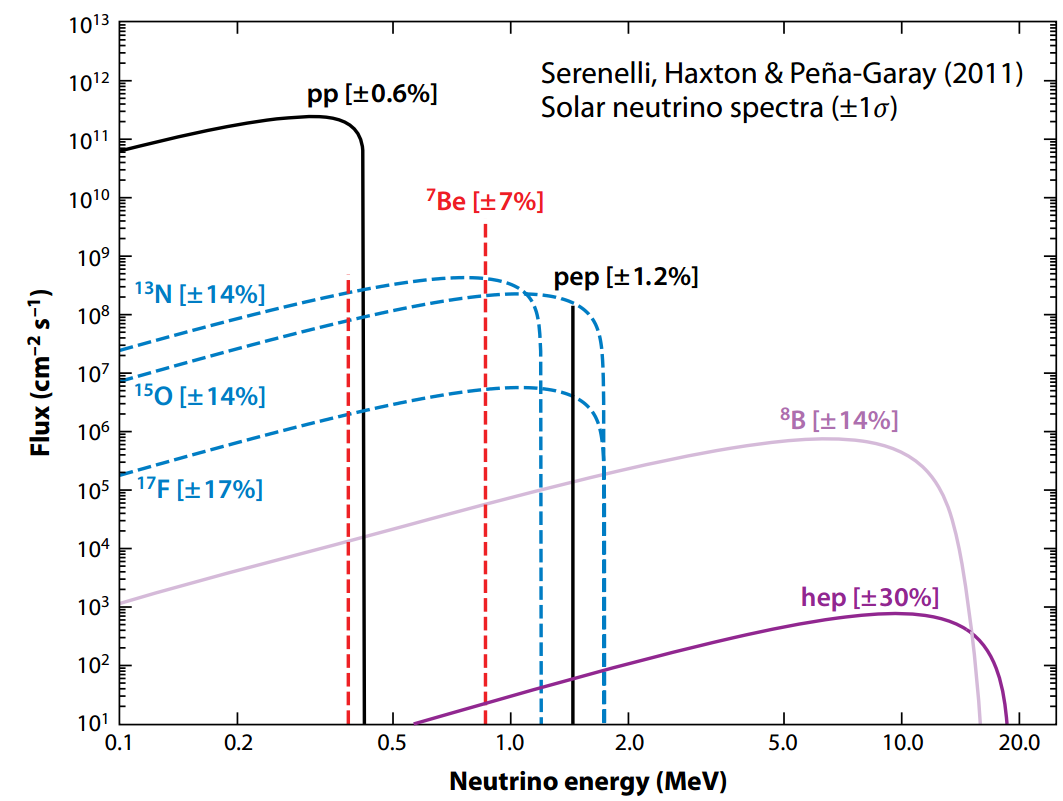
\includegraphics[width=12cm]{haxton09.png}
	\caption[Solar neutrino energy spectrum.]{Solar neutrino energy spectrum ($E_\nu$ vs. flux) along with the SSM uncertainties, from Ref.~\cite{haxton2013solar}.}
	\label{fig:haxton2013plot}
\end{figure}
In 1964, J. Bahcall and R. Davis proposed the first experiment to detect solar neutrinos \cite{bahcall1964solar,davis1964solar}. Davis designed an experiment that used a 380 m$^3$ tank filled with Perchloroethylene (C$_2$Cl$_4$), a dry-cleaning fluid rich in chlorine. Solar neutrinos were expected to change $^{37}$C1 to $^{37}$Ar via the endothermic reaction: $\nu_e+^{37}$Cl$\to^{37}$Ar$+e^-$, and the resulting $^{37}$Ar atoms were extracted and counted (a `radiochemical' method). The neutrino energy threshold ($E_{\mathrm{min}}$) of the experiment was 0.814 MeV, which allowed a measurement mostly of the $^8$B solar $\nu_e$ flux but also including some lower energy neutrinos \cite{davis1964solar}. Their first results, announced in 1968, showed that only about one-third of the predicted radioactive argon atoms were measured\cite{davis1968search}. This pioneering experiment raised a problem of the ``missing'' solar neutrinos, the ``solar neutrino problem.''

\subsection{Kamiokande and Super-Kamiokande}\label{sect:superKsolarnu}

The solar neutrino problem was later confirmed by the Kamiokande-II experiment in 1988 \cite{superKwebsite}. As the successor of the Kamiokande, Super-K uses a 50-kilotonne water Cherenkov detector to measure the solar neutrinos via the $\nu+e^-$ elastic scattering. By utilizing the pattern of Cherenkov light produced by the recoil electrons (see Sect.~\ref{sect:cherenkov}), the direction of the incoming neutrino can be traced and thus neutrinos produced specifically by the sun can be selected. Unlike the radiochemical method, this enables real-time measurements of the solar neutrinos.

In 2000, Super-K reported the observed solar neutrino flux to be only about 45\% of the flux expected according to the SSM, and with more than a 99.9\% confidence level. This suggest there had been a flavor transformation of solar neutrinos, and limited the oscillation parameters ($\Delta m^2_{21}$, $\theta_{12}$) \cite{superKwebsite}. 

Super-K continues to measure solar neutrinos with more precision and higher statistical accuracy, and the energy threshold has been lowered to 3.5 MeV to enable a search for $^8$B solar neutrinos. The fourth phase of Super-K (Super-K-IV) took data from 2008 to 2014, and by utilizing this 1664 live-day data, Super-K-IV reported a measurement of the elastic scattering flux as: $\Phi_{ES}=(2.308\pm0.020(stat.)^{+0.039}_{-0.040}(syst.))\times 10^6~\mathrm{cm^{-2}s^{-1}}$\cite{abe2016solar}. Combined with the previous three phases, it gives $\Phi_{ES}=(2.345\pm0.014(stat.)\pm 0.036(syst.))\times 10^6~\mathrm{cm^{-2}s^{-1}}$\cite{abe2016solar}. In Chapter 6 these values will be compared to the SNO+ measurements of this thesis.

\subsection{SNO}

The Sudbury Neutrino Observatory (SNO) experiment finally resolved the solar neutrino problem and first confirmed that the missing solar neutrinos are due to the neutrino flavor transformation $\nu_e\to\nu_{\mu,\tau}$, along with the matter effect mentioned in Sect.~\ref{sect:MSW}. 

SNO used a 1-kilotonne heavy water (D$_2$O) Cherenkov detector to distinguish the flavors of solar neutrinos. The SNO detector was sensitive to the $^8$B solar neutrinos via three interactions: (1) the charged current (CC) on deuteron ($d$): $\nu_e+d\to p+p+e^-$, (2) the neutral current (NC): $\nu_x+d\to p+n+\nu_x$, and (3) the elastic scattering (ES): $\nu_x+e^-\to \nu_x+e^-$. The CC channel was sensitive only to $\nu_e$ while the NC channel was independent of the neutrino type (``flavor-blind''), which provided a measurement of the total solar neutrino flux regardless of neutrino flavors. The ES channel was also sensitive to all flavors but with reduced sensitivities to $\nu_\mu$ and $\nu_\tau$ \cite{ahmad2002direct}. As mentioned in Sect.~\ref{sect:NuEStheory}, from Eqn.~\ref{eq:ratio1} the ES cross-section of $\nu_e$ is 6.5 times larger than that of $\nu_{\mu,\tau}$ (combined). 

In 2002, SNO reported that the measured total $^8$B solar neutrino flux via the NC channel ($\Phi_{NC}$) was consistent with the SSM while the $\nu_e$
component of the flux ($\Phi_e$) was about one-third of the total flux\cite{ahmad2002direct}:
\begin{equation}
R = \Phi_{CC}/\Phi_{NC} = \Phi_e/\Phi_{tot}=0.34\pm 0.04.
\end{equation}

A combined analysis of SNO data acquired from 1999 to 2006 gave the measured total flux of $^8$B solar neutrinos as $\Phi_{^8\mathrm{B}}=5.25\pm0.16(stat.)^{+0.11}_{-0.13}(syst.)$ cm$^{-2}$s$^{-1}$. Based on a two-flavor neutrino oscillation analysis, SNO implied that $\Delta m^2_{21}=(5.6^{+1.9}_{-1.4})\times 10^{-5}$ eV$^2$ and $\tan^2\theta_{12}=0.427^{+0.033}_{-0.029}$ \cite{aharmim2013combined}.

\subsection{KamLAND}

As mentioned in Sect.~\ref{sect:VacuumOsci}, reactor antineutrino experiments study the neutrino flavor transformation by measuring $\mathcal{O}$(MeV) $\bar{\nu}_e$ produced by nuclear reactors. If the distance between the reactor and the detector is long enough (according to Eqn.~\ref{oscillationCondition}, $L\sim\mathcal{O}(100$~km)), such experiments can probe the $\Delta m^2_{12}$ and $\theta_{12}$ parameters, or the flavor transformation parameters in the solar sector. KamLAND is able to study the solar sector due to its long baseline of 180 kilometers (the average value of the distances to the various reactors). It is a 1-kilotonne liquid scintillator detector, located in Gifu Prefecture, Japan, under Mount Ikenoyama at a depth of about 2700 metres water equivalent ($m.w.e$) \cite{abe2008precision}. KamLAND measures the $\bar{\nu}_e$ via the inverse beta-decay (IBD) process $\bar{\nu}_e + p \rightarrow n + e^+$, utilizing the prompt (light) signal produced by annihilation of the positron $e^+$, along with the delayed
coincidence with the signal due to the $\gamma$ emitted by neutron capture on a nucleus after thermalization \cite{pdg2020}. KamLAND provided best fit values of \cite{gando2011constraints}: $\Delta m_{21}^2=7.50^{+0.19}_{-0.20}\times10^{-5} \; \mathrm{eV^2}$ and $\tan^2\theta_{12}=0.452^{+0.035}_{-0.033}$. This value for $\tan^2\theta_{12}$ matches well with the solar neutrino measurements, but for the $\Delta m^2_{21}$ there is a $<2\sigma$ level tension, which may be attributable to statistical fluctuation or some minor effect, such as the day/night matter effect.

Assuming CPT invariance, the KamLAND and solar neutrino data can be combined by including solar $\nu_e$ and reactor $\bar{\nu}_e$ data to obtain the oscillation parameters. These values have been given in Sect.~\ref{sect:VacuumOsci}.

\subsection{Borexino}

Borexino is a liquid scintillator neutrino detector with a target mass of about 300 tonnes. It is located at the Gran Sasso National Laboratory (LNGS) in central Italy, under an overburden of rock with 3800 water equivalent meter (m.w.e) to suppress the cosmogenic backgrounds. It is the first experiment to have made real-time measurements of low energy ($<1$ MeV) solar neutrinos, thanks to the high light yield of the liquid scintillator \cite{agostini2020improved}.

Unlike a water Cherenkov detector, although a liquid scintillator provides more (detectable) photons per unit of neutrino energy deposited, it cannot be used to measure the event direction (see Sect.~\ref{sect:scintillator}). Borexino mainly measures the energy spectrum of the recoil electrons from the $\nu+e^-$ ES, a method that is termed `spectroscopic' \cite{agostini2020improved}. Precise measurements of the energy spectrum can identify different types of solar neutrinos and separate backgrounds.

Borexino has measured the $^7$Be, pep, pp and $^8$B solar neutrino fluxes \cite{agostini2018comprehensive}. In 2020 it reported the first observation of CNO neutrinos with an interaction rate of $7.2^{+3.0}_{-1.7}$ counts per day per 100 tonnes of target at 68\% C.L., and this result gives an estimate of the CNO neutrino flux at the Earth as $7.0^{+3.0}_{-2.0}\times 10^8 \; \mathrm{cm^{-2} \, s^{-1}}$ \cite{borexino2020experimental}. An improved measurement of the $^8$B solar neutrino was reported in 2020, with the elastic scattering flux (integrated over energy range $3.2<E_\nu <17$ MeV) determined as $\Phi_{ES}=(2.57^{+0.17}_{-0.18}(stat.)\pm 0.07 (syst.))\times 10^6 \; \mathrm{cm^{-2} \, s^{-1}}$ \cite{agostini2020improved}.

\subsection{More Studies on Solar Neutrino and Future Experiments}\label{sect:futureSolar}

There are at least the following three avenues for future solar neutrino research: (1) precision measurements of solar neutrino fluxes, (2) sub-leading-order effects on the phenomenology from both standard and nonstandard physics, and (3) new detection techniques \cite{antonio2018state}.

Currently, $hep$ neutrinos have not been measured yet due to the weakness of their flux. On the other hand, although most `species' of low energy solar neutrinos have been discovered (i.e. measured), more precise measurements would help to probe the details of matter effects, measure the oscillation parameters in the solar sector more precisely to resolve the tensions between reactor- and solar-source experiments, and could unveil new physics such as nonstandard neutrino interactions (NSI) by observing sub-leading effects \cite{gann2015everything}. Among the low energy neutrinos, pep neutrinos enjoy the distinction of being mono-energetic (with $E_\nu$=1.442 MeV), and their flux is well predicted by the Standard Solar Model \cite{davini2016cno}. A precise measurement of the pep neutrinos will give more information on the matter effect in neutrino oscillations. 

Solar metallicity ($Z$) is the abundance of elements heavier than $^4$He (called ``metal'' elements in the context of astronomy). It is poorly constrained and the predictions from different solar models vary. Since the sub-dominant CNO neutrino flux depends linearly on the metallicity of the solar core, a precise measurement of the CNO neutrinos can determine the abundance of $^{12}$C, $^{13}$N and $^{15}$O in the Sun and thus determine the solar metallicity \cite{cerdeno2018cno}.

Several new experiments using various detection techniques are being planned, to precisely measure the solar neutrinos in the near future. These experiments include:

Large-scale water Cherenkov detectors, such as Hyper-Kamiokande (Hyper-K). Hyper-K is the next generation of Super-K, and it is designed to have a fiducial mass of 187 kilotonnes, about $8 \times$ larger than that of Super-K. With a 4.5-MeV energy threshold, it will measure the $^8$B solar neutrinos, and it expects to observe 130 $\nu+e^-$ elastic scattering events per day. With such a high count rate, the oscillation parameters in the solar sector can be precisely measured. Hyper-K also has a potential to detect the $hep$ neutrinos\cite{yano2019solar}. 

A liquid argon neutrino detector, such as DUNE (Deep Underground Neutrino Experiment), can provide two channels for detecting solar neutrinos: $\nu_e+^{40}$Ar$\to e^-+^{40}$K$^*$ and the $\nu+e^-$ ES process: $\nu_x+e^-\to\nu_x+e^-$. Similar to Hyper-K, DUNE aims for precise measurements of $^8$B neutrinos, and also searches for $hep$ neutrinos \cite{capozzi2019dune}.

Large-scale liquid scintillator detectors with $\mathcal{O}(10)$ kilotonne fiducial mass, such as ASDC (Advanced Scintillation Detector Concept)-THEIA \cite{askins2020theia}, JUNO (Jiangmen Underground ) \cite{giaz2018status}, Jinping (Jinping Neutrino Experiment) \cite{beacom2017physics}, and LENA (Low Energy Neutrino Astronomy) \cite{wurm2013studying}, are expected to be built to measure low energy solar neutrinos. Some new liquid scintillator techniques (such as water-based liquid scintillator) will be implemented to precisely measure neutrino energy and incoming direction. More details of the water-based liquid scintillator will be discussed in Sect.~\ref{sect:wbWLS}, Chapter 3.

Ton-scale dark matter direct search experiments, such as the DARWIN experiment (DARk matter WImp search with liquid xenoN) can also measure low-energy solar neutrinos. With an energy threshold down to several keV and ultra-low background level, DARWIN will be able to measure the pp and $^7$Be solar neutrinos \cite{baudis2014neutrino,aalbers2016darwin,aalbers2020solar}.

SNO+, one of the operating large-scale liquid scintillator detectors, has measured the $^8$B solar neutrino flux during its initial water phase \cite{anderson2019measurement}. In the following (scintillator) phase, SNO+ is able to measure low energy solar neutrinos ($E_\nu<2$ MeV), and specifically the CNO and $pep$ neutrinos. Due to the depth of SNOLAB, SNO+ is expected to have much lower cosmogenic backgrounds than did Borexino, and thus may obtain more precise measurements \cite{directorReview}. More details will be discussed in Sect.~\ref{sect:scintPhase}, Chapter 3.

\section{Neutrinoless Double Beta Decay}\label{sect:doublebeta}

The neutrino flavor transformation experiments proved that neutrinos are not massless. However in these experiments mass {\em differences} rather than absolute masses are measured, so we cannot from these results know the absolute scale of neutrino mass. Currently, there are three main approaches to probing the neutrino masses \cite{valle2015neutrinos}: (1) Cosmological measurements \cite{aghanim2020planck,dvorkin2019neutrino,lesgourgues2013neutrino}; (2) Direct measurements of the $\beta$-decay spectrum; and (3) A search for the neutrinoless double beta decay ($0\nu\beta\beta$) process, which will be discussed below.

For heavy radioactive isotopes ($A>70$) whose nuclei have even neutron number and even proton number (``even-even'' nuclei), beta decay results in an odd-odd daughter nucleus that is {\em less} stable. Thus for such isotopes, the $\beta$-decay is energetically forbidden. In 1935, M. Goeppert-Mayer pointed out that these isotopes can still decay through a {\em double} beta decay process: $(Z,A) \to (Z+2,A)+2e^{-}+2\bar{\nu}_e+Q_{\beta\beta}$, where $Q_{\beta\beta}$ is the released energy. This is called ordinary double beta decay or $2\nu\beta\beta$, which is allowed within the SM. Typically the half-life for isotopes subject to $2\nu\beta\beta$ $T_{1/2}>10^{19}$ years (yr) \cite{povh2008particles,martin2019nuclear}.

In the SM, neutrinos are neutral (charge 0) fermions. As such, there is no apparent quantum number to distinguish a neutrino and an antineutrino\cite{akhmedov2014majorana}. A neutral fermion that {\em is} its own antiparticle is named a `Majorana' particle, in honour of E. Majorana who developed a mathematical modification of the Dirac equation\cite{majorana2006symmetric}.

In 1939 W.H.Furry \cite{furry1939transition} proposed that {\em if} neutrinos are Majorana particles (Majorana neutrinos), then a process called neutrinoless double beta decay ($0\nu\beta\beta$) will also be expected to occur: $(Z,A) \to (Z+2,A)+2e^{-}+Q_{\beta\beta}$. In this process, evidently the {\em lepton number changes} 2, which within the scope of the SM is not allowed. Should such a decay be observed, a new paradigm for elementary particle physics will be required. The Feynman diagrams for $2\nu\beta\beta$ and $0\nu\beta\beta$ are compared in Fig.~\ref{fig:feynman}.
\begin{figure}[htbp]
	\centering
	{
	\subfigure[$2\nu\beta\beta$.\label{fig:feynman:2nubb}]{
		\begin{minipage}[t]{0.45\textwidth}
			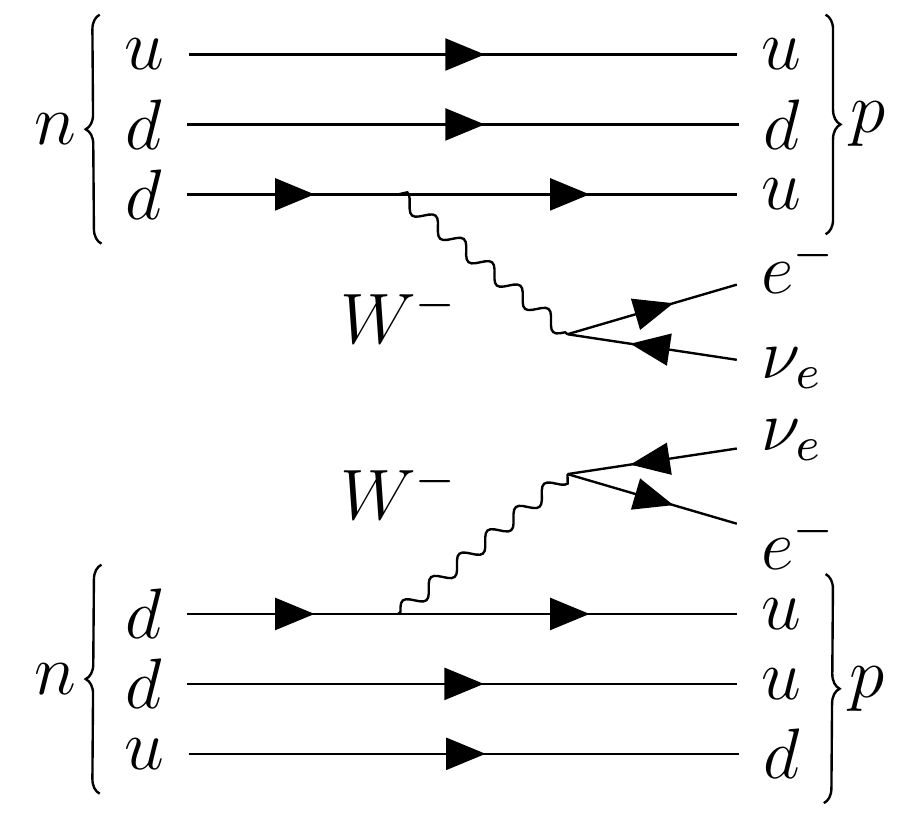
\includegraphics[width=5cm]{doubleBeta2nu_feynman.png}
		\end{minipage}
	}
	\subfigure[$0\nu\beta\beta$.\label{fig:feynman:0nubb}]{
		\begin{minipage}[t]{0.45\textwidth}
			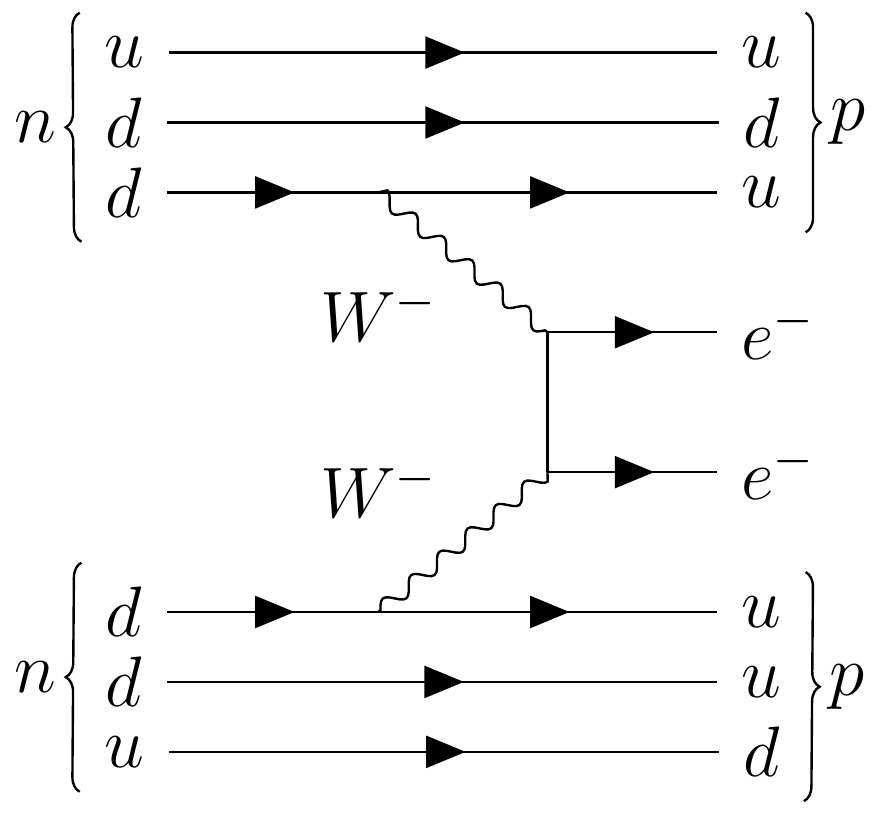
\includegraphics[width=5cm]{doubleBeta_feynman.png}
		\end{minipage}
	}
		\caption[Feynman diagrams for $2\nu\beta\beta$ and $0\nu\beta\beta$.]{Feynman diagrams for $2\nu\beta\beta$ (a) and $0\nu\beta\beta$ (b).		\label{fig:feynman}}
	}
\end{figure}

For the Majorana neutrino, an effective Majorana mass $\langle m_{ee}\rangle$ is defined as \cite{suekane2015neutrino,zuber2020neutrino}:
\begin{equation}\label{eq:effective_nuMass}
\langle m_{ee}\rangle = |\sum_{i=1}^3 U^2_{ei}m_i|= |c^2_{13}c^2_{12}m_1+c^2_{13}s^2_{12}e^{i\alpha_1}m_2+s^2_{13}e^{i\alpha_2}m_3|,
\end{equation}
where the values of $U_{ei}$ are the elements of the neutrino mixing matrix for the flavor state $\nu_e$, and $m_i$ are the mass eigenvalues of the mass eigenstates, according to Enq.~\ref{eq:mixingmatrix}; $\alpha_1,\alpha_2$ are two Majorana CP-violation phase factors ranging from 0 to $\pi$, and $\alpha_2$ can also be taken as $\alpha_2-\delta_{CP}$.

The neutrino mass eigenvalues $m_i$ can be expressed as the lightest neutrino mass $m_{\nu \mathrm{min}}$ and mass square differences $\Delta m^2_{ij}$\cite{suekane2015neutrino}. For the normal hierarchy (NH),
\begin{eqnarray*}
m_{\nu \mathrm{min}} &=& m_1 \; , \\
m_2 &=& \sqrt{m_{\nu \mathrm{min}}^2+\Delta m^2_{21}} \; , \\
m_3 &=& \sqrt{m_{\nu \mathrm{min}}^2+|\Delta m^2_{31}|} \, ,
\end{eqnarray*}
while for the IH, 
\begin{eqnarray*}
m_{\nu \mathrm{min}} &=& m_3 \; , \\
m_1 &=& \sqrt{m_{\nu \mathrm{min}}^2+|\Delta m^2_{31}|} \; , \\
m_2 &=& \sqrt{m_{\nu \mathrm{min}}^2+|\Delta m^2_{31}|+\Delta m^2_{21}} \; .
\end{eqnarray*}
In this case, the effective Majorana mass can be derived from $m_{\nu \mathrm{min}}$ and neutrino flavor transformation parameters $\theta_{ij}$ and $\Delta m^2_{ij}$. A probe of the effective Majorana mass $\langle m_{ee}\rangle$ can thus determine $m_{\nu \mathrm{min}}$ and (in turn) the absolute neutrino masses. 

The decay width and the half-life of the $0\nu\beta\beta$ process are calculated as \cite{suekane2015neutrino,zuber2020neutrino}:
\begin{equation}\label{eq:decayWidth0vbb}
\Gamma=(T^{0\nu}_{1/2})^{-1} = G_{PS}(Q,Z) \; |M_{Nuc}|^2 \; \langle m_{ee}\rangle^2, 
\end{equation}
where $G_{PS}(Q,Z)$ is a phase space corresponding to the effective coupling constant, which depends on the endpoint energy $Q$ and the atomic number $Z$, while $|M_{Nuc}|$ is the nuclear matrix element describing the nuclear transition. The latter can be calculated theoretically, albeit using {\em approximate methods} based on many-body nuclear models, such as the Nuclear Shell Model (NSM), interacting Boson Model (IBM), etc. Since $G_{PS}$ and $|M_{Nuc}|^2$ can be calculated theoretically, a $0\nu\beta\beta$ experiment measures $T^{0\nu}_{1/2}$ to quantify $\langle m_{ee}\rangle$.

Similar to the $\beta$-decay case, the $2\nu\beta\beta$ process will cause a continuous spectrum in the detector. However very significantly, the (hypothetical) $0\nu\beta\beta$ process only has {\em two electrons in the final state} and so the {\em sum of the energies of these two electrons is constrained}. These electrons must carry away the total energy released by the decay (the energy from the nuclear recoil is negligible here), and so a spectrum of the (summed) energy released to the outgoing electrons must show a distinct energy peak at the Q-value ($Q_{\beta\beta}$). Taking the isotope $^{130}$Te as an example, Fig.~\ref{te130energy} illustrates the shapes of the energy spectrum from the $2\nu\beta\beta$ and the $0\nu\beta\beta$ decay processes.
\begin{figure}[htbp]
	\centering	
	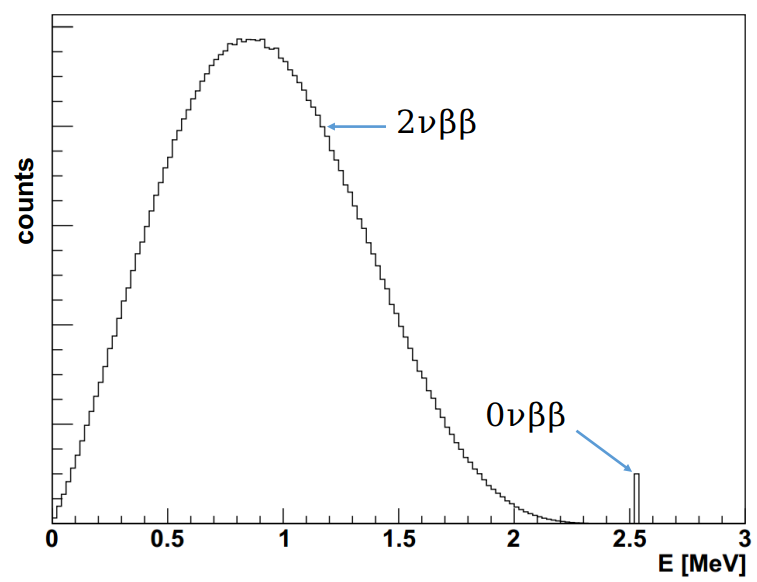
\includegraphics[width=8cm]{Te130_energy0vbb.png}
	\caption[Energy spectrum of the $^{130}$Te $2\nu\beta\beta$ decay and the hypothetical $0\nu\beta\beta$ decay.]{Energy spectrum of the $^{130}$Te $2\nu\beta\beta$ decay and the hypothetical $0\nu\beta\beta$ decay (sum of the energies of the two outgoing electrons). The SNO+ software package (\texttt{RAT}) was used to produce the simulations for the plot. The package is described in Sect.~\ref{sect:rat}.}
	\label{te130energy}
\end{figure}

To determine $T^{0\nu}_{1/2}$, experiments search for events in which the total energy deposited is close to $Q_{\beta\beta}$. For a candidate isotope, the observed number of events in expectation is: 
\begin{equation}
N_{event} = \ln 2 \; \frac{N_A}{M_A} \; \frac{\alpha\cdot\epsilon\cdot m\cdot t}{T^{0\nu}_{1/2}},
\end{equation}
where $N_A$ is the Avogadro's number, $\alpha$ is the abundance of the isotope in the element, $M_A$ is the molar mass of the isotope, $m$ is the target isotope mass in the detector, and $t$ is the measurement time of total exposure.

There are 35 candidate isotopes that can undergo the $2\nu\beta\beta$ decay process, but only a few of them are suitable for the application in direct $0\nu\beta\beta$ search experiments \cite{giunti2007fundamentals}. From the experimental viewpoint, the candidate isotopes are expected to have relatively high natural abundances and high Q-values, be deployable in a large amount with low cost, be atoxic and unharmful to the environment, etc. However, in a realistic situation, no isotope fulfills all these criteria, and trade-offs have to be made for contemporary experiments \cite{dolinski2019neutrinoless}. Fig.~\ref{fig:te_abundance} shows the Q-values and natural abundances of the candidate isotopes currently selected by the $0\nu\beta\beta$ experiments.

\begin{figure}[!htb]
	\centering
	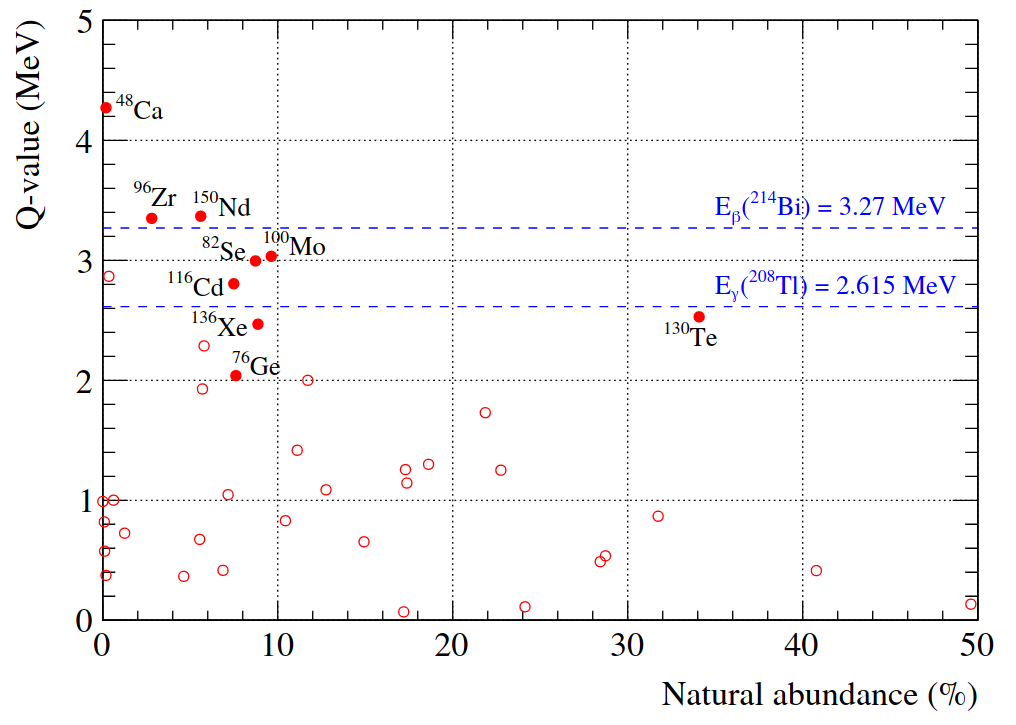
\includegraphics[width=10cm]{Te_abundance.png}
	\caption{Natural abundance vs. Q-values for different $2\nu\beta\beta$ isotopes, from Ref.~\cite{snop_nim_draft}.}
	\label{fig:te_abundance}
\end{figure}

Among the isotopes under consideration, $^{130}$Te has the highest natural abundance of 34\% and thus can provide a higher target isotope mass. SNO+ will use Te-loaded liquid scintillator to search for $0\nu\beta\beta$, which will be discussed in Chapter 3. 

At the time of this writing, no experiment has found the signal of $0\nu\beta\beta$, while limits on $T^{0\nu}_{1/2}$ and $\langle m_{ee}\rangle$ for various candidate isotopes have been set. Currently, the best limit on $T^{0\nu}_{1/2}$ reported by the experiments is obtained from the KamLAND-Zen Experiment, searching for the signal from the $^{136}$Xe. Their 2016 results gave a lower limit of $T^{0\nu}_{1/2}(^{136}$Xe$)>1.07\times 10^{26}$ yr at 90\% C.L., and a corresponding upper limit on the effective Majorana mass: $\langle m_{ee}\rangle<(61-165)$ meV \cite{gando2016search}. 

For $^{130}$Te, the current best limit is from the CUORE experiment (Cryogenic Underground Observatory for Rare Events). In 2018, CUORE placed a lower limit of $T^{0\nu}_{1/2}(^{130}$Te$)>1.5\times 10^{25}$ yr at 90\% C.L., with $\langle m_{ee}\rangle<(110-520)$ meV \cite{alduino2018first}.

For $^{76}$Ge, the current best limit is from the GERDA experiment (GERmanium Detector Array). In 2019, GERDA reported a lower limit half-life of $T^{0\nu}_{1/2}(^{76}$Ge$)>1.8\times 10^{26}$ years at 90\% C.L. with $\langle m_{ee}\rangle<(79-180)$ meV \cite{agostini2020final}.

Future experiments such as the KamLAND2-Zen, LEGEND-1000 and nEXO, coming to fruition within about a decade, are required to reach $T^{0\nu}_{1/2}$ at $\mathcal{O}(10^{27}-10^{28})$ years \cite{dolinski2019neutrinoless}.

